\documentclass[10pt]{article}

\pagestyle{plain}
\textheight 9in
\textwidth  6.5in
%\footheight 0.0cm
\topmargin  0pt
\headheight 0in
\headsep 0in
\leftmargin 0.0cm
\oddsidemargin  0cm
\def\baselinestretch{1.0}
\parindent 0.0 cm
\parskip   0.2 cm

\newcounter{step}
\newtheorem{theorem}{Theorem}
\newtheorem{proposition}{Proposition}
\newtheorem{corollary}{Corollary}
\newtheorem{definition}{Definition}

\renewcommand{\floatpagefraction}{0.90}
\renewcommand{\topfraction}{0.90}
\renewcommand{\bottomfraction}{0.90}
\renewcommand{\textfraction}{0.10}

\def\thesection{\large{\arabic{section}.}}
\def\thesubsection{\normalsize{\thesection\arabic{subsection}}}
\def\thesubsubsection{\normalsize{\thesection\arabic{subsection}.\arabic{subsubsection}}}
\usepackage{float}
\usepackage[dvips,xetex]{graphicx}
\begin{document}

\newpage
\thispagestyle{empty}
\begin{center}
{\Large \textbf{ Multi-Layer Infrastructure Repairs in a Post-Disaster Context}} \\
\vspace*{0.2cm}
%{\large \textbf{Brian French and Erhan Kutanoglu}} \\
%{\large \textbf{Operations Research and Industrial Engineering Program}} \\
%\large \textbf{The University of Texas at Austin}} \\
%{\large \textbf{Austin, TX 78712, USA}} \\
%{\large \textbf{BCFrench@utexas.edu, erhank@mail.utexas.edu}} \\
\end{center}

\thispagestyle{empty}
\begin{center}
{\large \bf Abstract}
\end{center}
Both power and road networks sustain major damage in the wake of hurricanes. Repair efforts should therefore consider the interactions between the two networks. This paper introduces several frameworks based around models for both power and road repair and uses them to demonstrate the impacts of coordinating repairs. These models are run on several scenarios using IEEE power grid standards to provide computational examples. Results show that full coordination between power and road repair agencies is more effective than reduced coordination combined with post processing.



{\large \bf Keywords}\\
\vspace*{-12pt}

\vspace*{-12pt}
\section{{\large Introduction}}
\label{sec:ic:intro}
\vspace*{-12pt}

Hurricanes provide a growing concern in the operation of power grids in coastal areas. This paper was undertaken to address the gap in the literature where previous efforts don't consider how network layers depend on each other. To affect  repairs on a damaged power grid element, the element must be accessible to the crew attempting to repair it, which implies that the road grid is a part of the repair efforts. In the process of a hurricane, the road grid will sustain substantial damage from flooding and debris on the road surface, which necessitates road grid repairs/clearance as well. To handle the issues of repairing power grids efficiently, consideration for repairs of both aspects should be considered jointly. Previous literature doesn't study this specific interaction as discussed below.
\vspace*{-12pt}
\subsection{\large Existing Literature}
\vspace*{-12pt}
Damage from hurricanes on infrastructure elements is well studied. All of \cite{WinklerEA2010}, \cite{ScherbEA2015}, and \cite{GuikemaEA2010} have looked at the damage to power grids in varying capacities and methodologies. Damage to the road network is studied more in the context of repairing damage. \cite{AksuEA2014} addresses concerns of accessibility to locations in the wake of road damage. \cite{DuqueEA2016} focuses their work on the ability to move disaster supplies around.

In the context of power grid repair, it comes from two major areas: Network interdiction and work similar to this paper. \cite{SalmeronEA2010} is a paper emblematic of work on interdiction and provide the basis for the linear programming formulation of DC power flow used in this paper.  \cite{NPSMasters} addresses a problem similar to this work, though without addressing travel times at all. \cite{ArabEA2015} and \cite{MousavizadehEA2018} both address repairs to power grids in the context of resilience. Most similar to this paper is \cite{BentEA2011} in that they consider DC power flow and repair with travel times jointly. The key distinction is that they presume that the road operates under nominal conditions rather than including repair of the road grid into the problem.
\vspace*{-12pt}
\section{\large{Model}}
\vspace*{-12pt}
\subsection{Overview}
The problem to be addressed is how to handle interactions between road and power networks during disaster response. We choose to do this by solving the problems independently to keep runtime tractable and then testing a variety of post processing methods to handle the interactions. This should allow us to capture which interactions are worth the effort to address and which can be ignored in the name of preserving runtime or simplifying analysis. 
\subsection{Assumptions}
\vspace*{-12pt}
While considering coordinated repair using the mixed-integer programs below, we assume complete information about damage to both networks, complete information about repair times, and no variation in repair times. In the course of modeling the problem, we assume that a DC-flow model of power grid operation is close enough to real network behavior to draw useful insights \cite{QiEA2012}. We also assume in the power grid repair model that a minimum spanning tree can approximate routing elements as the minimum spanning tree provides a bound on the traveling salesman problem and therefore routing problems.
\subsection{Road Model}
\vspace*{-12pt}
To model the road repair aspect of the problem, we choose to treat it as a problem of routing a crew tasked with clearing debris and flooding from roads. In doing this, damaged roads aren't rendered unable to be transited, but their lengths are merely increased to account for the difficulty traversing them while clearing debris, minor flooding, and the like. This problem is handled by solving a variation of the prize collecting rural postman problem at each time step. The discrete time here is done to match up with both standard shift lengths and the discrete time requirement of the DC power flow based model for the power grid.

Defining Parameters and Sets to begin:
\begin{displaymath}
$$
$\begin{array}{ll}
T & \mbox{the set of time periods (shifts) over the time horizon}\\
N & \mbox{the set of nodes in the graph}\\
C_{ij} & \mbox{ measure of the value of the road from i to j}\\
L_{ij} & \mbox{is the length of the road between nodes $i$ and $j$ when everything is working as normal}\\
R_{ij} & \mbox{time to repair the road between $i$ and $j$}\\
I_{ij} & \mbox{initial condition of the road between $i$ and $j$}\\
\end{array}$
$$
\end{displaymath}
Next Defining Decision Variables
\begin{displaymath}
$$
$\begin{array}{ll}
X_{ij}^t & \mbox{binary indicator for road $ij$ being operational in time t}\\
K_{ij}^t & \mbox{binary indicator for travel from $i$ to $j$ being in the tour at time $t$}\\
S_{ij}^t & \mbox{Length of travel for road $ij$ at time $t$}\\
\end{array}$
$$
\end{displaymath}


We then elect to minimize the length of non functioning road over the repair horizon. Without loss of generality the objective can be replaced with the repair priority weights for an agency of choice. 
\begin{equation}
	\min \sum_{t \in T}  \sum_{i,j \in N} C_{ij}*(1-X_{ij}^t) 
\end{equation}
	
	
	\mbox{Subject To:}
	
	\begin{eqnarray}
	\sum_{i,j \in N} S_{ij}^t K_{ij}^t \leq 8, \hspace{6pt} \forall t\in T \\
	S_{ij}^t = \max \{L_{ij}, (1-X_{ij}^t)R_{ij} \}, \hspace{6pt} \forall t\in T \hspace{4pt} \forall i,j \in N\\
	\sum_{j \in N} K_{ij}^t - \sum_{j \in N} K_{ji}^t = 0, \hspace{6pt} \forall t\in T \hspace{4pt} \forall i \in N\\
	X_{ij}^t \le \sum_{t'=0}^{t-1} K_{ij}^{t'} + I_{ij}, \hspace{6pt} \forall t\in T \hspace{4pt} \forall i,j \in N\\
	\sum_{i,j \in S; i\neq j} X_{ij}^t \leq |S|-1 \hspace{6pt} \forall S \subset N; \hspace{2pt} S \neq \emptyset
	\end{eqnarray}
Constraint (2) is a shift scheduling constraint capping the length of each tour. Constraint (3) is a linearizable representation of the length of a road conditional on its repair status where a road that has yet to be repaired costs the repair time to transit and a repaired road can be transited at its nominal time. Constraints (4) and (6) are standard routing constraints for subtour elimination and path connectivity. Constraint(5) defines the working of damaged roads.


\subsection{Power Model}
\vspace*{-12pt}
To model the power repair aspect of the problem, we treat it primarily as a scheduling problem. This repair schedule is subject to travel time and shift length constraints, which complicate things as well as an embedded DC power-flow model to evaluate each shift. Traditional routing problems are computationally intractable with commercial solvers on this scale, so to keep runtime in check, a spanning tree was used instead as it provides a lower bound on routing and therefore captures most of the tradeoffs \cite{Held1971}. We model this in discrete time windows for the sake of allowing easier interaction between the two related problems, but also for handling DC power flow on a power grid as there is no simple way to implement continuous runtime DC power grids with binary repair decisions.

We begin modeling the power half of the problem by defining the relevant parameters, sets, and design variables:

\small
\begin{displaymath}
$$
$\begin{array}{llll}
	 N & \mbox{set of nodes, indexed by $i$} & X_{e}^{t} & \mbox{flow on line $e$ at time $t$}\\
	 E & \mbox{set of power lines, indexed by $e$} & G_{k}^t & \mbox{production from generator $k$ at time $t$}\\
	 R & \mbox{the set of road segments} & V_i^t & \mbox{indicator for node $i$ functioning at time $t$}\\
	 T & \mbox{the planning horizon, indexed by t} & W_{e}^t & \mbox{indicator for line $e$ functioning at time $t$} \\
	 O(i) & \mbox{set of lines with origin i} & S_{e}^t & \mbox{indicator for line $e$ serviced at time $t$}\\
	 D(i) & \mbox{set of lines with destination i} & F_i^t & \mbox{indicator for node $i$ serviced at time $t$}\\
	 o(e) & \mbox{origin node of line e} & \theta_i^t & \mbox{hase angle for the power flow at $i$ in time $t$}\\
	 d(e) & \mbox{destination node of line e} & MST_t & \mbox{length of the tree used for "routing" at $t$} \\
	 \underline{L_e},\overline{L_e} & \mbox{capacity lower and upper bounds for the power line $e$}& Z_{ij}^t & \mbox{indicator for $i$ to $j$ in the spanning tree at $t$}\\
	 \Delta_{i} & \mbox{time to repair node $i$} \\
	 \delta_{e} & \mbox{time to repair line $e$}\\
	  C_{SP(i)} & \mbox{length of the shortest path to node $i$ from the central depot}\\
	  D_i & \mbox{power demand at location $i$ in the pre-disaster steady state}\\
	  P_k & \mbox{maximum power generation for generator $k$}\\
	  B_e&  \mbox{line susceptance for power line $e$}\\
	 I_e, I_i & \mbox{initial condition of line $e$ and node $i$, respectively}
\end{array}$
$$
\end{displaymath}
\normalsize
The model is then as follows
\begin{equation}
\min \sum_{i \in N} \sum_{t \in T} (1-W_i^t)D_i
\end{equation}
subject to:
\begin{eqnarray}
 X_e^t = B_e * (\theta_{o(e)}^t - \theta_{d(e)}^t), \hspace{5pt} \forall t \in T, \hspace{4pt} \forall e \in E\\
 G_i^t - \sum_{l \in O(i)} X_l^t + \sum_{l \in D(i)} X_l^t = D_i, \hspace{4pt} \forall t \in T, \hspace{4pt} \forall i \in N\\
 G_k^t \leq P_{k} V_{k}^t, \hspace{4pt} \forall t \in T, \hspace{4pt} \forall k \in N\\
 \underline{L_e}W_{e}^t \leq X_{e}^t \leq \overline{L_e}W_{e}^t, \hspace{4pt} \forall t \in T, \hspace{4pt} \forall e \in E\\
 \underline{L_e}V_{o(e)}^t \leq X_{e}^t \leq \overline{L_e}V_{o(e)}^t, \hspace{4pt} \forall t \in T, \hspace{4pt} \forall e \in E\\
 \underline{L_e}V_{d(e)}^t \leq X_{e}^t \leq \overline{L_e}V_{d(e)}^t, \hspace{4pt} \forall t \in T, \hspace{4pt} \forall e \in E\\
 MST^t = \sum_{i \in N} \sum_{j \in N} SP_{ij}^t*Z_{ij}^{t} C_{speed}\hspace{4pt} \forall t \in T\\
 \sum_{i \in N} \sum_{j \in N} Z_{ij}^{t} = \sum_{i \in N} F_i^t + \sum_{e \in E} S_e^t - \sum_{i \in N} F_i^t \sum_{O(i)} S_e^t - \sum_{i \in N} F_i^t \sum_{D(i)} S_e^t \hspace{4pt} \forall t \in T\\
 \sum_{i,j \in S} Z_{ij}^t \leq |S|-1 \hspace{4pt} S\subset N\\
 \sum_{j \in N} Z_{ij}^t \leq F_i^t + \sum_{e \in O(i) \cup D(i)} S_{e}^t \hspace{4pt} \forall t \in T\hspace{4pt} \forall i \in N \\
 \sum_{e \in E} \delta_{e}S_e^t + \sum_{i \in N}\Delta_{i}F_i^t + MST_t <=8\\
 V_i^t \leq \sum_{t'=0}^{t-1} F_i^{t'}+I_i, \hspace{4pt} \forall i \in N\\
 W_{e}^t \leq \sum_{t'=0}^{t-1} S_{e}^{t'}+I_e, \hspace{4pt} \forall e \in E
 \end{eqnarray}
 Constraints (8)-(13) define the flow on a damaged power grid with load being either switched on or switched off at a demand node under standard DC flow conditions. The binary condition of load at nodes is done to account for the last mile distribution lines being damaged at first making partial load shedding unrealistic. Constraints (14)-(17) handle construction of a minimum spanning tree(MST) between nodes being repaired during a shift to approximate the routing cost. Constraint (15) is an inclusion/exclusion constraint to ensure the MST is constructed between the right set of nodes. We assume that a power line can be fixed starting from either of it's endpoints. Constraint (18) defines shift scheduling to limit the amount of work to what fits in a shift , and constraints (19) and (20) handle constraining operation to elements that are working.
\section{\large{Results}}
\vspace*{-12pt}
\subsection{Methods}
 \vspace*{-12pt}
 
 To demonstrate both validity and utility of the model, we generate two test cases, one based on the IEEE 30 bus network and a second based on the IEEE 57 bus network. Both power grids were overlaid with a Watts-Strogatz graph to provide an simulation of a road network for the sake of the routing aspects of the problem. \cite{Watts1998} \cite{Newman2002}. To generate a damage scenario, a subset of geographically co-located nodes, power lines, and road network edges were marked as damaged to have scenarios to solve.
 
 The scenarios were each solved under the following frameworks:
 \vspace{-8pt}
 \begin{itemize}
 	\item Solve the road repair problem and use the solution to generate a time varying shortest path matrix for use when solving the power repair problem. This makes as few assumptions as possible without solving a multiobjective problem. This is functionally an iterative solution where the road grid repair actor moves first and the power repair actor solves their problem in response to that.
 	\item Solve the power repair problem assuming statically damaged roads. This assumes no information about the road repair schedule and generates the best schedule possible under that assumption.
 	\item Solve the power repair problem assuming nominal road conditions and add a one-shift delay to account for the road repairs getting completed done before the roads are needed. This is an iterative solution equivalent to solving the power grid problem first and forcing the road actor to solve with conditions imposed by roads needed for power repair.
 	\item Solve the power repair problem without travel time and using the generated schedule, post process it into a feasible repair schedule. Post processing is done by solving a knapsack problem heuristically by adding the lowest cost repair including travel time with the requirement that the repair can't occur before it does in the no-travel time solution
 \end{itemize}
\vspace{-8pt}
Using the above method, the schedule without travel times can be used to provide a bound both time to repair as well as minimum load shed at each iteration. The repair model with constantly damaged roads provides an upper bound on lost demand over the planning horizon with action being taken immediately.
%%frameworks?
%%lower bound with schedule
%%upper bound with non-interacting road damage
%%iterative
\subsection{IEEE 30 Bus Case}

The IEEE 30 bus network is a standard test/example power grid that is based on the power grid in southern Illinois in the 1960s . More importantly, it's been a well understood standard test grid since it's inception. We mark approximately 50\% of the road and power edge elements as damaged and about 25\% of the nodes corresponding to power grid substations and demand areas as damaged. For a second scenario, we mark 75\% of edges as damaged and 40\% of nodes to show that the results hold regardless of damage level.
\begin{figure}[H]
	\centering
	\caption{Load Shed by shift in the 30 Bus case}
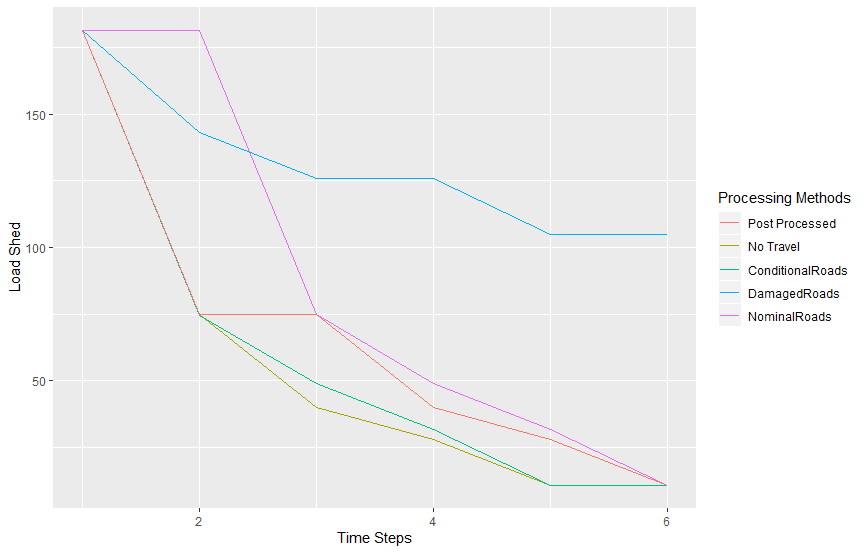
\includegraphics[width=.75\textwidth, height=0.5\textheight,keepaspectratio]{Rplot37.png}

\end{figure}
\begin{figure}[H]
	\centering
	\caption{Load Shed by shift in the 30 Bus case in a second scenario}
	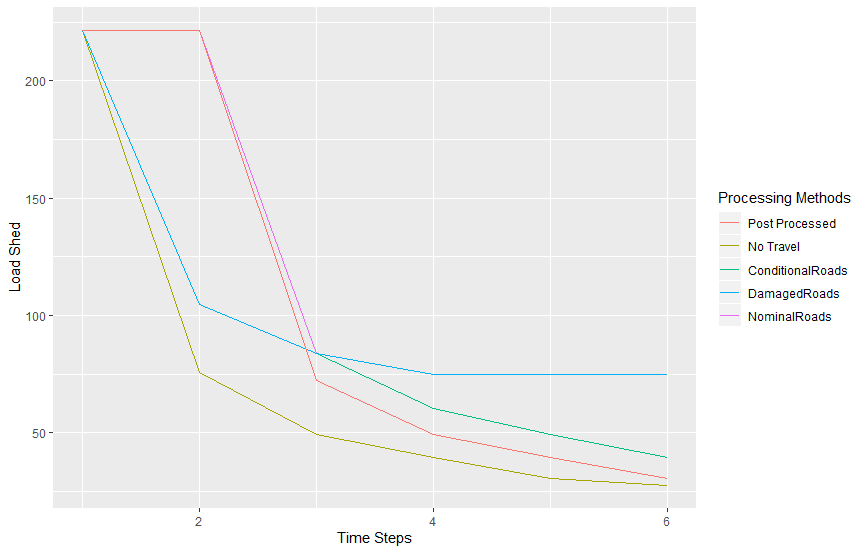
\includegraphics[width=.75\textwidth, height=0.5\textheight,keepaspectratio]{Rplot30Scenario2.png}
	
\end{figure}
The above figure suggests that increased coordination between repair actors improves the rate at which power can be restored. This is largely intuitive, but suggest that revision in processes for handling post-hurricane relief can be improved. The repair schedule generated from conditioning is closest to the lower bound in both scenarios (357.7 MW-shifts of unserviced demand vs 345.4 in the first scenario. 559.4 vs 444 in the higher damage scenario). The post-processed schedule presumes nominal road operation which would in practice mean that the power utility can dictate the road repair schedule and road clearing starts far enough ahead that any road needed by the power utility to affect repairs is traversable at it's nominal runtime by the time it's needed. Given this, we conclude that coordinated repair is better than a best-case post processed schedule and is closer to the optimal way to treat the problem.
\subsection{IEEE 57 Bus Case}
The setup for this case/scenario is nearly identical to the setup for the 30 bus case above, but with a different power grid in order to demonstrate that differences in repair schedules aren't due to overfitting to a topology. The IEEE 57 bus network topology is another standard test network based on part of the American Electric Power System in the Midwestern US. Similar amounts of damage is applied to this network before the system was solved out.

\begin{figure}[H]
	\centering
	\caption{Load Shed by shift in the 57 Bus case}
	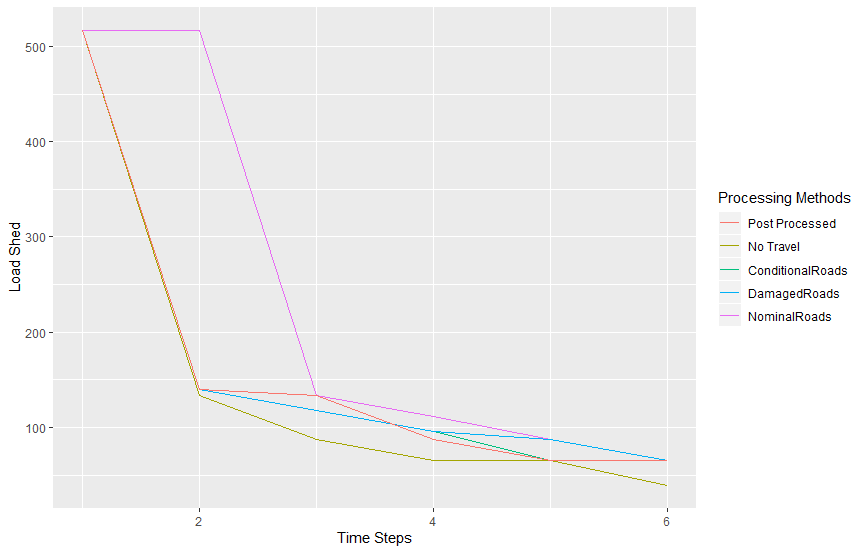
\includegraphics[width=.75\textwidth, height=0.5\textheight,keepaspectratio]{RPlot57.png}
	
\end{figure}

Again we draw similar conclusions. More coordination once more leads to faster repairs of the power grid. The difference here is that the post-processed schedule with nominal condition roads is better than the conditioned solution method for one time segment rather than being always better. That said, the iterated repair method still has a lower summed loss over its planning horizon than the best possible case of post processed schedule (936.8 vs 943.1 MW-shifts of unserviced power demand). These results are similar to both scenarios from the 30 bus case allowing us to conclude that solving road and power repair iteratively is better than trying to handle the power problem alone and the post-process into a valid repair schedule.
\section{\large{Conclusions}}
\label{sec:issues}
\vspace*{-12pt}

From this, we can draw the conclusion that increasing levels of model complexity representing an improved fidelity to fully coordinated operations yields lower levels of demand shed. This suggests that at a practical level the agency responsible for restoration of the road grid should keep the agency responsible for the power grid informed of their plans as well as the state of the road network in order to more quickly restore power after a disaster.
\bibliographystyle{plain}
\bibliography{sources}

\end{document}
